% !TeX root = 01_main.tex
% !TEX program = xelatex
% !BIB program = biber

\documentclass[12pt, a4paper]{report}	
% Formatierungen und Packages
\usepackage{fontspec}
\usepackage[ngerman]{babel}% Language setting
\usepackage[
  a4paper,
  top=2cm,
  bottom=2cm,
  left=2.5cm,
  right=2.5cm,
  headheight=20pt,
  headsep=15pt
]{geometry} % Set page size and margins
\usepackage{graphicx} % Required for inserting images
%\usepackage{amsmath}
\usepackage{xcolor}
\usepackage{csquotes} % \enquote nutzen zum Zitieren \enquote 
\usepackage{fancyhdr}
\usepackage{setspace}
\usepackage{titlesec}
\usepackage{comment}
\usepackage{booktabs}
\usepackage{tabularx}
\usepackage{array}
\usepackage{pdfpages}
\usepackage{acronym}
\usepackage[
    backend=biber,
    style=authoryear,
    dashed=false,
    url=false
]{biblatex}
\usepackage{xurl} % sorgt für automatische Zeilenumbrüche bei zu langen Links im Quellenverzeichnis
\usepackage{tocbibind}
\usepackage{tocloft}
\usepackage{enumitem}
\usepackage{nameref}
\usepackage{chngcntr} % \counterwithout figure chapter
\usepackage{threeparttable}
\usepackage{caption}
\usepackage[colorlinks=true, allcolors=blue, hypertexnames=false]{hyperref} % allcolors=black setzen am Ende um Links zu schwärzen
% hypertexnames=false Verhindert doppelte PDF-Anker und fehlerhafte Sprungziele bei
% zurückgesetzten Seiten-, Kapitel- oder Abbildungszählern.
\usepackage{cleveref}

%\excludecomment{figure} % damit werden auf einem Schlag alle Abbildungen ausgeblendet
%\usepackage{showframe}
%\usepackage{layout}
\setmainfont{Arial}
%\setlength{\bibhang}{0pt} % Einzug im Quellenverzeichnis deaktivieren
\DeclareDelimFormat{labelnamepunct}{\addcolon\space}
\DeclareFieldFormat{url}{\url{#1}}
\DeclareBibliographyDriver{online}{%
    \usebibmacro{bibindex}%
    \usebibmacro{begentry}%
    \printnames{author}%
    \setunit{\addcolon\space}%
    \printfield{title}%
    \setunit{\addperiod\newline}%
    \printtext{In:\space}%
    \printfield{url}%
    \iffieldundef{urlyear}
    {}
    {~\mkbibparens{%
     \printfield{urlday}.%
     \printfield{urlmonth}.%
     \printfield{urlyear}%
   }}%
   \nopunct
    \usebibmacro{finentry}%
}
\DeclareBibliographyDriver{unpublished}{%
    \usebibmacro{bibindex}%
    \usebibmacro{begentry}%
    \printnames{author}%
    \setunit{\addcolon\space}%
    \printfield{title}%
    \setunit{\addcomma\space}%
    \printdate
    \printtext{
    \mkbibparens{%
    \printfield{note}%
    }
    }%
    \nopunct
    \usebibmacro{finentry}%
}
% \setlength{\headheight}{20pt} % Fehler hat gesagt Headheight größer
% \addtolength{\topmargin}{-5pt} % Befehl ist um Text weiter hoch zu schieben wegen \headheight{17.01598pt} (es müsste eigentlich 15pt sein)

\setstretch{1.3}
\titleformat{\chapter}[hang]
    {\fontsize{14pt}{22pt}\selectfont\bfseries} % Format
    {\thechapter.} % Label
    {1em} %Abstand
    {} % <Vor-Code>
\titleformat{\section}[hang]
    {\fontsize{14pt}{18pt}\bfseries} % Format
    {\thesection} % Label
    {1em} %Abstand
    {} % <Vor-Code>
\titleformat{\subsection}[hang]
    {\fontsize{12pt}{18pt}\bfseries} % Format
    {\thesubsection} % Label
    {1em} %Abstand
    {} % <Vor-Code>
\titlespacing*{\chapter}{0pt}{-26pt}{12pt}
\DeclareNameFormat{nurNachname}
  {\MakeUppercase{\namepartfamily}}
  
\DeclareCiteCommand{\footdirekt}[\mkbibfootnote] % Zitat direkt
  {}
  { \printnames[nurNachname]{author},
    \printfield{year},~\printfield{postnote}\nopunct}
  {}
  {}
\DeclareCiteCommand{\footvgl}[\mkbibfootnote] % Vergleich Zitat
  {}
  { vgl. \printnames[nurNachname]{author}, \printfield{year},~\printfield{postnote}\nopunct}
  {}
  {}
\DeclareCiteCommand{\footonline}[\mkbibfootnote]
  {}
  {
    online:
    \printnames{author},
    \printdate,
    \mkbibparens{%
      \printfield{urlday}.%
      \printfield{urlmonth}.%
      \printfield{urlyear}%
    }%
    \nopunct
  }
  {}
  {}
\DeclareCiteCommand{\footunpub}[\mkbibfootnote] % Vergleich Zitat
  {}
  { vgl. unveröffentlicht: 
  \printnames[nurNachname]{author}, 
  \printdate
  \nopunct
  }%
  {}
  {}
\newcommand{\abschnitt}[1]{%
  \paragraph{#1}\mbox{}\par
}
\counterwithout{figure}{chapter} % Kapitelnummer bei Abbildungen entfernen, fortlaufende Nummerierung
\counterwithout{table}{chapter} % Kapitelnummer bei Tabellen entfernen, fortlaufende Nummerierung
\counterwithout{footnote}{chapter} % fortlaufende Nummerierung der Fußnoten bei Kapitelwechsel, sonst Reset bei Kapitelwechseö
\captionsetup[figure]{
    labelfont=bf,
    labelsep=space,
    justification=raggedright,
    singlelinecheck=false,
    format=hang
}
\captionsetup[table]{
    labelfont=bf,
    labelsep=space,
    justification=raggedright,
    singlelinecheck=false,
    format=hang
}
\newcommand{\fullref}[1]{Tabelle \ref{#1} \enquote{\nameref{#1}}}
\addbibresource{literatur.bib}
\begin{document}
%\layout
\setlength{\parindent}{0pt} % Einzug nach Bildern im gesamten Dokument deaktivieren
\renewcommand{\cftchapleader}{\cftdotfill{\cftdotsep}} % Punkte im Inhaltsverzeichnis
\setlength{\cftbeforetoctitleskip}{0pt} % Höhe vor Inhaltsverzeichnis
\setlength{\cftbeforeloftitleskip}{0pt} % Höhe vor Bilderverzeichnis
\setlength{\cftbeforelottitleskip}{0pt} % Höhe vor Tabellenverzeichnis
\setlength{\cftafterloftitleskip}{12pt} % Höhe nach Abbildungsverzeichnis
\setlength{\cftafterlottitleskip}{12pt} % Höhe nach Tabellenverzeichnis
\setlength{\cftaftertoctitleskip}{12pt} % Höhe nach Inhaltsverzeichnis
\renewcommand{\cfttoctitlefont}{\Large\bfseries} % Größe Überschrift Inhaltsverzeichnis
\renewcommand{\cftloftitlefont}{\Large\bfseries} % Größe Überschrift Abbildungsverzeichnis
\renewcommand{\cftlottitlefont}{\Large\bfseries} % Größe Überschrift Tabellenverzeichnis
\fancypagestyle{projektarbeit}{
    \fancyhf{} % Kopf- und Fußzeile leeren
    \fancyhead[R]{\colorbox{yellow}{Vorname Nachname}}
    \fancyhead[L]{\nouppercase{\leftmark}}
    \fancyfoot[R]{\thepage}
}
\fancypagestyle{plain}{ % Das ist für die Kapitelanfangsseiten
    \fancyhf{} % Kopf- und Fußzeile leeren
    \fancyhead[R]{\colorbox{yellow}{Vorname Nachname}}
    \fancyhead[L]{\nouppercase{\leftmark}}
    \fancyfoot[R]{\thepage}
}
\fancypagestyle{anhang}{
    \fancyhf{} % Kopf- und Fußzeile leeren
    \fancyhead[R]{Anhang \thechapter}
    \fancyhead[L]{\nouppercase{\leftmark}}
    \fancyfoot[R]{\thepage}
}
\renewcommand{\chaptermark}[1]{% Kommentar bis zum Zeilenende“. Hier werden sie verwendet, um unerwünschte Leerzeichen zu verhindern.
  \markboth{\thechapter.\ #1}{}%
} % Entfernen des Wort Kapitels in der Kopfzeile
% Verzeichnisse
\pagenumbering{Roman}
% !TeX root = ../01_Projektarbeit/01_main.tex
\begin{titlepage}

\centering

\vspace{1cm}

{\Huge\bfseries Projektarbeit 1\par}

\vspace{1cm}

{\Large
Beispieltitel einer 
Beispielarbeit
Beispielschlusswort
\par}

\vspace{1cm}

\begin{tabular}{p{5cm}p{9cm}}
\textbf{Eingereicht am:} & 
\colorbox{yellow}{XX.XX.XXXX} \\[0.5em]
\textbf{Von:} &
\textbf{Max Mustermann} \\
&
Musterstraße 37g\\
&
34612 Musterort \\[1em]
\textbf{Studiengang:} &
Digital Engineering \\[1em]
\textbf{Seminargruppe:} &
DE25-1 \\[1em]
\textbf{Matrikelnummer:} &
400XXXX \\[1em]
\textbf{Praxispartner:} &
Musterfirma \\
&
Musterstraße 3 \\
&
34612 Musterort \\[1em]
\textbf{Gutachter:} &
Chef Musterperson \\
&
(Musterfirma) \\
&
Musterprofessor \\
&
(Duale Hochschule Sachsen Glauchau)
\end{tabular}
\end{titlepage}
 % Titelseite
    \clearpage
\begin{enumerate}[nosep]
	\item Hier muss der Themenvorschlag für die Projektarbeit eingebunden werden, direkt pdf als 02\_Themenblatt in 02\_Kapitel speichern bitte
	\item siehe Quelltext 01\_main.tex: Zeile 170
	\item siehe nächste Zeile im Quelltext  \verb|\includepdf|
	\item nach einfügen der pdf kann dieses enumerate entfernt werden
\end{enumerate}
%\includepdf[pages=1]{../02_Kapitel/02_Themenblatt} % Hier Themenvorschlag für die Projektarbeit einbinden
\clearpage
\pagestyle{projektarbeit}
\tableofcontents
    \clearpage
\listoffigures
    \clearpage
\listoftables
    \clearpage
\chapter*{\vspace{12pt}Abkürzungsverzeichnis}
\addcontentsline{toc}{chapter}{Abkürzungsverzeichnis}
    \vspace{12pt}
\begin{acronym}[Abkürzunggg] % Länge dieses Strings 'Abkürzunggg' legt Platz zwischen Acro und Langform fest
	\acro{Beispielacro}{Ausgeschriebene Abkürzung}
\end{acronym}
\clearpage
\pagenumbering{arabic} % Arabische Numerierung der Seitenzahlen


%Fließtext
% !TeX root = ../01_Projektarbeit/01_main.tex
\chapter{Einleitung / erstes Kapitel}
\acresetall % damit wird die Verwendung von allen Akronymen zurückgesetzt

\section{Erstes Unterkapitel}
Hier kommt der Text für die Aufgabenstellung herein.

\section{Zweites Unterkapitel}
Hier kommt Text für die Zielstellung herein.

    \clearpage
% !TeX root = ../01_Projektarbeit/01_main.tex
\chapter{How To / Anleitung}

Für einen Abschnitt nutzt man \verb|\abschnitt| (selbstdeklarierter Befehl in 01\_main.tex)

\abschnitt{Anleitung}

Zum \textit{kursiv} schreiben nutzt man \verb|\textit{}|
\newline

Um Akronyme einzufügen, müssen diese vorher selbstständig in 01\_main.tex deklariert werden.
\newline

Zitierstil für Kommentare muss noch geändert werden da in der Fußnote folgendes erscheint: "NACHNAME, 2026," > nach dem Jahr steht ein unnötiges Komma.
\newline

Um eine neue Zeile zu beginnen, muss man im Quellcode eine LEERZEILE lassen.
\newline

\verb|\newline| für eine Textumbruch ohne Formatierung der Zeile.
\newline

\verb|\linebreak| für einen Textumbruch bei dem die Zeilenfüllung formatiert wird bzw. richtet den Text als Blocksatz aus
\newline

für eine leerzeile schreibt man \verb|\\| am ende der zeile und drückt dann 2x Return
\verb|\enquote| für Zitate wie z.\,B. \enquote{Hallo}, man kann auch \verb|\enquote| in einem \verb|enquote| benutzen: \enquote{Hier ist noch ein \enquote{enquote} drin}
\newline

für z.\,B. nutzt man \verb|z.\,B| also: z.\,B
\newline

mit einem \verb|\label{eigene bezeichnung:eigener labelname}| kann man einen verlinkung setzen z.\,B. hier mit label abschnitt:unterkapitel, für die Referenz nutzt man \linebreak \verb|~\ref{abschnitt:unterkapitel}|. z.\,B. so hier: Siehe Kapitel ~\ref{abschnitt:unterkapitel}
\newline

Wenn man Einträge in literatur.bib ändert oder eine neue Fußnote schreibt muss man immer ein mal biber laufen lassen
\newline

Arten von Fußnoten / Auflistung mit Zahlen:
\begin{enumerate}[nosep]
	\item \verb|\footvgl[Seite der Quelle]{Name der Quelle in literatur.bib}|: für indirekte Zitate\footvgl[34]{Buch1}
	\item \verb|\footdirekt[Seite der Quelle]{Name der Quelle in literatur.bib}|: für direkte Zitate\footdirekt[3]{Buch3}
	\item \verb|\footonline{Name der Online-Quelle in literatur.bib}|: für Zitate aus Online-Quellen\footonline{OnlineQuelle1}
	\item \verb|\footunpub{Name des Dokuments/Quelle in literatur.bib| für unveröffentlichte Dokumente\footunpub{intern}
\end{enumerate}
Die Fußnoten sind selbstständig definierte Befehle, zu finden in 01\_main.tex.
\newline

Auflistung mit Stichpunkten:
\begin{itemize}[nosep, label=-]
	\item erster Stichpunkt
	\item zweiter Stichpunkt
	\item mit Label stellt man das Stichpunktzeichen ein\newline
\end{itemize}

Abstände im Abbildungsverzeichnis sind größer wenn sich die Abbildungen in unterschiedlichen Kapiteln befinden.
\newline

Wenn ein Akronym \enquote{Underfoll box} verursacht kann man das nehmen:

\verb|\setlength{\emergencystretch}{1em}% ACRO sorgt für underfull box|


\clearpage

\section{Unterkapitel Beispiel}
\label{abschnitt:unterkapitel}
Beispieltext mit Beispielakronym: \ac{Beispielacro}.Referenz zu dem Bild einer kleinen Mieze: Abbildung~\ref{fig:Kitten Eins}. Dieser Satz endet mit einer Fußnote\footvgl[24]{Buch1}.
\begin{figure}[htbp]
	\centering
	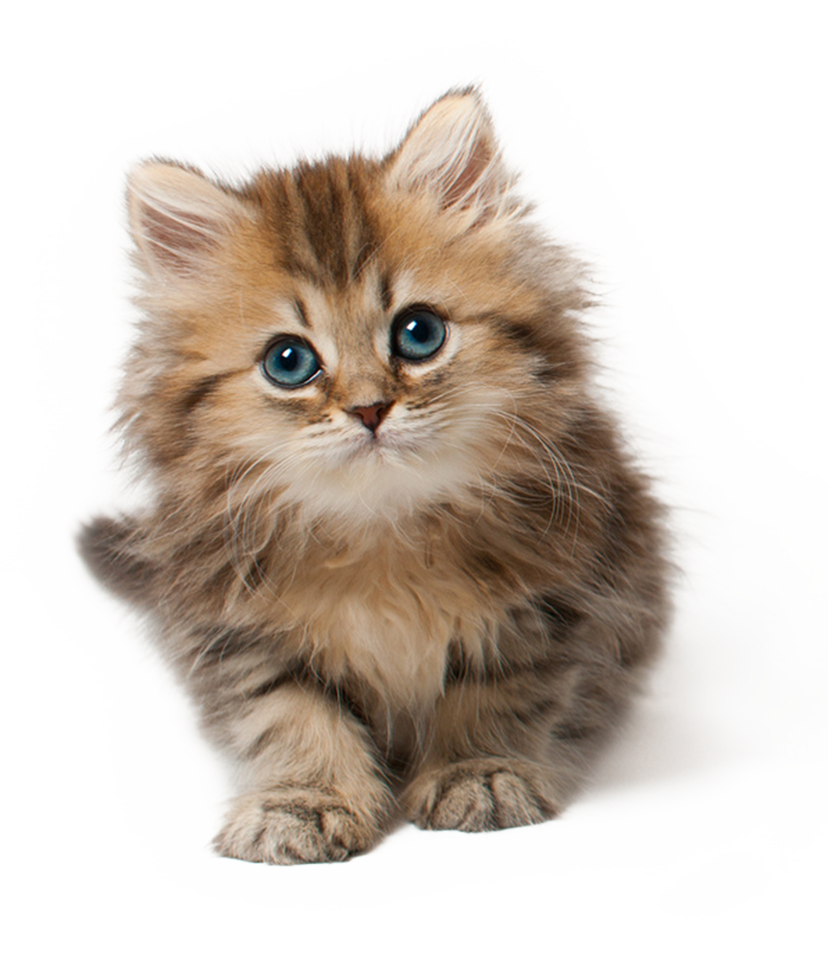
\includegraphics[width=0.5\textwidth]{../03_Bilder/kitten_1.jpg}
	\caption[Süßes Kätzchen 1]{Süßes Kätzchen 1

	{\fontsize{10}{12}\selectfont (Eigene Darstellung)}}
	\label{fig:Kitten Eins}
\end{figure}

Tabelle~\ref{tab:Beispieldaten} zeigt eine Beispieltabelle:
\begin{table}[htbp]
	\centering
	\renewcommand{\arraystretch}{1.3}
		\begin{tabular}{l|l}
			\textbf{Beispielspalte 1} & \textbf{Beispielspalte 2} \\
			\hline
			Spaltentrennung wird mit \verb|&| gemacht -> &
			um in die nächste Zeile zu gehen nutzt man \verb|\\| \\
			\hline
			So kann man hier &
			schöne Sachen hereinschreiben \\
			als Label wurde hier &
			\verb|label{tab:...}| verwendet
		\end{tabular}
		\caption[Beispieldaten]{%
			Beispieldaten\\
			{\fontsize{10}{12}\selectfont (Fiktiv)}%
		}
		\label{tab:Beispieldaten}
\end{table}
\clearpage

    \clearpage

% Quellen und Anhänge
\printbibliography[title={Quellenverzeichnis}] % Quellenverzeichnis ausgeben
\addcontentsline{toc}{chapter}{Quellenverzeichnis} % Quellenverzeichnis zu Gliederung hinzufügen
\appendix % ab hier werden kapitel mit buchstaben nummeriert
\renewcommand{\thechapter}{\arabic{chapter}}
\chapter*{Anhangsverzeichnis}
\addcontentsline{toc}{chapter}{Anhangsverzeichnis}
\begin{table}[htbp]
    \renewcommand{\arraystretch}{1.5}
    \begin{threeparttable}
        \begin{tabular}{@{}p{2.5cm}l}
            \hyperref[anh:default]{Anhang 1} & \hyperref[anh:default]{default} \\
        \end{tabular}
        \label{tab:Test}
    \end{threeparttable}
\end{table}
\titleformat{\chapter}[hang]
    {\fontsize{14pt}{22pt}\selectfont\bfseries} % Format
    {Anhang \thechapter} % Label
    {1em} %Abstand
    {} % <Vor-Code>
\renewcommand{\chaptermark}[1]{% Kommentar bis zum Zeilenende“. Hier werden sie verwendet, um unerwünschte Leerzeichen zu verhindern.
  \markboth{#1}{}%
} % Entfernen des Wort Kapitels in der Kopfzeile

% Ab hier können Anhänge eingefügt werden
\pagestyle{anhang}
\clearpage
\setcounter{page}{1}
% !TeX root = ../01_Projektarbeit/01_main.tex
\chapter{default}
\thispagestyle{anhang}
\label{anh:default}

Für jeden Anhang am besten eine eigene .tex erstellen und Labels setzen.

Hier können dann .pdf oder images eingefügt werden

    \clearpage
\end{document}
